%-------------------------------------------------------------------------------
%	CAPITOLO 31
%-------------------------------------------------------------------------------

\chapter{In pretura - 12 scudi all'avvocato - Sentenza per donne - Interrogatorio - Un Testimonio - Due asinelli}
\subsection{In pretura}
La pretura, sotto il Papa, era nel \index[Luoghi]{Borghetto}Borghetto, nella casa \index[Luoghi]{Lanconelli (palazzo)}Lanconelli ora \index[Luoghi]{Martini (palazzo)}Martini e precisamente sopra lo spaccio. Nello spaccio e camera retrostante vi erano le prigioni.\\
\indent L'attuale camera dello spaccio era la prigione, larga, dove i prigionieri attraverso la finestra dell'orto, parlavano liberamente col pubblico, chiedevano la carità, mettevano fuori una sporta che i passanti riempivano di cibi.

\subsection{12 scudi all'avvocato}
L'avvocato \index[Personaggi]{Baldrati Girolamino (avvocato)}Girolamino Baldrati, della famiglia ancora esistente dei Cavaler, aveva la fama di tirar fuori i prigionieri, ed a lui affluivano i clienti. \\
\indent Un giorno, parlava attraverso la finestra con un contadino d'Umana, carcerato e suo cliente, al quale esponeva le difficoltà di tirarlo fuori, poi concluse: <<Ti garantisco di tirarti fuori, ma ho delle spese, bisogna che tu mi dia dodici scudi.>>\\
\indent Il contadino dopo i soliti stiracchiamenti contrattuali dovè chinare la testa e promettere all'avvocato di fargli tenere anticipati i chiesti dodici scudi.\\
\indent Tra la finestra superiore socchiusa, vi era il pretore a prendere il fresco, e ad ascoltare il colloquio.\\
\indent Partito che fu l'avvocato, questo pretore certo \index[Personaggi]{Amar\:.\:. d'Ferrara (pretore)}Amar\:.\:. d'Ferrara di famiglia illustre, chiamò \index[Personaggi]{Fantini}Fantini, custore delle carceri e gli ordinò di portargli su il contadino carcerato al quale disse: <<Sono io e non l'avvocato che ti deve liberare. Se mi dai i dodici scudi ti mando a casa subito, se no ti tengo dentro un pezzo.>>\\
\indent Il contadino: <<Propi am manda a ca?\footnote{<<Mi manda proprio a casa?>>}>>\\
\indent Pretore: <<Si, se mi dai i dodici scudi.>>\\
\indent Contadino: <<Alora a mend a dì a mi fradel cu mi purta\footnote{<<Allora mando a dire a mio fratello che me li porti>>}.>>\\
\indent Fu rimesso in carcere... in attesa. Intanto l'avvocato \index[Personaggi]{Baldrati Girolamino (avvocato)}Girolamino, non vedendo i dodici scudi andò alla solita inferiata della prigione, per sollecitarli dal cliente.\\
\indent Là seppe che il suo cliente era stato liberato senza processo e che i dodici scudi li aveva avuti il pretore... che finì col litigare con l'avvocato.

\subsection{Sentenza per donne}
Tre gentildonne dei \index[Luoghi]{Sabbioni}Sabbioni\footnote{Il \textbf{Borgo dei Sabbioni} era la zona attorno a via Saffi, dove vi era anche la villa della Marchesa, la quale venne sostituita nel dopoguerra da un condominio.} si erano querelate a vicenda innanzi al Pretore \index[Personaggi]{Pompaneri Demenego (pretore)}Pompaneri Demenego, da \index[Luoghi]{Conegliano Veneto}Conegliano Veneto.\\
\indent Questo pretore era un originale, un signore, girava in tuba e code\footnote{Le due code dei vestiti signorili dell'800.} per il paese, proprio quando la massa del popolo portava la `galoza'\footnote{Precisa Mingazzi: "Berretto di canapa/lana, per chi non lo sapesse"}.\\
\indent In udienza, Pretore ad una delle imputate: <<Cosa gasto ti?\footnote{<<Cos'hai fatto te?>>}>>\\
\indent Imputata: <<Mo signor la ma dé dla puténa\footnote{<<Ma signore, mi ha dato della puttana>>}\\
\indent All'altra imputata: <<E ti?\footnote{<<E te?>>}>>.\\
\indent Seconda imputata: <<Me aiò de dla puténa parchè lè steda lì la prèma\footnote{<<Io le ho dato della puttana perché è stata lei la prima a farlo>>}>>.\\
\indent Pretore alla terza imputata: <<E ti?>>\\
\indent Imputata: <<Sgnor che creda cagliè stedi lò dò a dem dla puténa pral premi e me aiò arspost\footnote{Signore creda che sono state le prime a darmi della puttana ed io ho risposto.>>}>>\\
\indent Pretore sentenzia indicando le imputate con un dito: <<Una, due, tre, tre putane fuori dei coioni tutte e tre!>>

\subsection{Un testimonio}
L'abate \index[Personaggi]{F\:.\:.\:. (abate)}F\:.\:.\:. aveva sparato collo schioppo contro il fiume ad un passero su di un albero.\\
\indent Per disgrazia andò ad impallinare vari ragazzi che erano a giocare sull'argine del fiume. L'unico testimonio era un povero vecchio, che non capiva troppo bene l'Italiano, non sapeva quel che si dicesse anche per la paura di trovarsi innanzi alla giustizia.	\\
\indent Il Pretore impazientito, al teste\footnote{Testimone}: <<C'eravate voi quanto l'abate ha sparato...>>\\
\indent Teste: <<Sgnor me ai zur che me ai sera, mo \emph{`c'eravate'} an lo visto in villo\footnote{<<Signore le giuro che c'ero, ma `c'eravate' non l'ho visto da nessuna parte>>.}>>.


\subsection{Interrogatorio}
\index[Personaggi]{Mamon}Mamon e \index[Personaggi]{Marturi}Marturi imputati.\\
\indent Pretore a Mamon: <<Che mestiere fate?>>\\
\indent \index[Personaggi]{Mamon}Mamon: <<Sgnor a feg e sansel, e gambarol, e sert, e barbir, e canzuler, e sbrazèt, a tus i chen...\footnote{<<Signore faccio il sensale, il gambarolo, il sarto, il barbiere, il calzolaio, toso i cani>>}>>.\\
\indent Pretore: <<Basta con questi mestieri>> - a Marturi - <<Che mestiere fate?>>\\
\indent \index[Personaggi]{Marturi}Marturi: <<Gnit sgnor\footnote{<<Nulla signore>>}>>.\\
\indent Pretore, brusco: <<Allora siete un vagabondo!>>\\
\indent Marturi: <<Sgnor, cosa vol ca fega e fa ignacosa lò!>> indicando \index[Personaggi]{Mamon}Mamon.\\
\indent Risata generale e la cosa è diventata un proverbio.

\subsection{Due asinelli}
La nostra \index[Luoghi]{Vincenzo Monti (piazza)}piazza\footnote{Piazza Vincenzo Monti} fu costruita nell'orto \index[Luoghi]{Camerani (palazzo)}Camerani\footnote{Nel 1848 come edificio per un nuovo municipio fu deciso l'acquisto della casa Camerani, una vecchia costruzione che si trovava di fronte all'attuale bar di piazza Monti (ex-Tavalazzi) e dell'orto annesso, che dava sulla via chiamata `Violina', perché molto stretta, che dal ponte andava (e va ancora oggi) fino al cosiddetto “Stradone della chiesa” (dal 1882 Corso Garibaldi). L'orto diventò l'attuale piazza, sistemata alla meglio cui fu dato il nome del poeta Vincenzo Monti\index[Personaggi]{Monti Vincenzo} e la Violina fu allargata e selciata con due marciapiedi laterali.}. Nei primordi era pressoché aperta e confinante con l'attigua campagna. Il nostro mercato della domenica, per le merci, e del lunedì, per merci e bestiame, era antico e cominciato fino dal 1700, per età accreditato ed in molto sviluppo quale centro urbano delle molte ville vicine. \\
\indent Mancavano i fabbricati ed in conseguenza i negozi, così che il commercio era disimpegnato dagli ambulanti. I mezzi di comunicazione erano povere strade, non imbrecciate\footnote{Non coperte con brecciame, ovvero pietrisco}, ed ancora più poveri traini, una carretta, con un ronzino, provato alle inginocchiature di S. Antonio\footnote{Provato fino allo stremo}, e sparuti asini. \\
\indent Come al solito i rivenditori legavano gli asini agli alberi della periferia della piazza, in mancanza di stalle o per economia.\\
\indent Un giorno due di questi asini, in fregola\footnote{Stato di eccitazione sessuale degli animali} d'amore si slegarono, fuggirono per la piazza, si fermarono nel maggiore spiazzo, costituito dalla bella mostra delle terraglie\footnote{Vasellame},  ben disposte dai venditori.\\
\indent In questi amori... la giumenta rimase sotto, abbracciata dalle gambe anteriori del maschio che la copriva... e non desistettero dal loro amplesso che a funzioni finite nonostante le randellate loro sferrate sui rispettivi musi.\footnote{Non fermarono l'amplesso se non quando ebbero finito, nonostante le botte sul muso che ricevevano}.\\
\indent Dei piatti... pestati ne rimasero i cocci. Di qui cominciò la lite tra i venditori delle terraglie ed i proprietari degli asini, per i risarcimenti. \\
\indent Il pretore \index[Personaggi]{C\:.\:.\:. (pretore)}C\:.\:.\:. sentenziò: <<Ritenuti i proprietari degli asini responsabili dei danni, doversi il proprietario dell'asino pagare metà dei danni, perché il suo asino aveva pestato e rotto i piatti con sole due zampe, il proprietario della giumenta dovere pagare il doppio del premio, per avere la sua bestia pestato e rotto le terraglie doppiamente con quattro gambe.>>\\
\indent Ai posteri... i commenti.

 \begin{figure}[htb]
    \centering
    \vspace{1cm}
    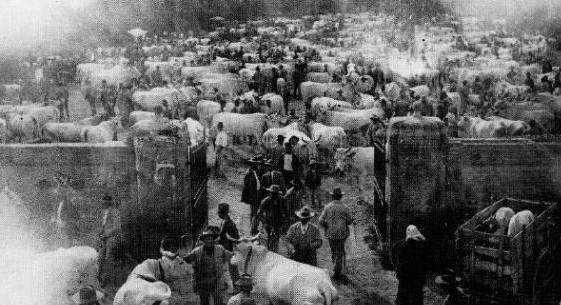
\includegraphics[width=\textwidth]{mercato}
    \caption[Mercato del Bestiame]{Il \textbf{mercato del bestiame}. Nel 1839 fu attrezzata un'area nuova per tale mercato: il \textbf{Campo Boario} `e marchè dal besti' in Corso Garibaldi, dove ora c'è la ditta Marini con i suoi capannoni\label{fig:mercato}}
    %\vspace{-0.3cm}
\end{figure}











%
